\documentclass[../mathNotesPreamble]{subfiles}

\begin{document}
%  \relscale{1.4} %TODO
  \section{5.1: Exponential Functions}
  
  \fbox{\parbox{0.9875\linewidth}{
    \textbf{Properties of Exponents:}
    \begin{itemize}
      \item If $m$ is a positive integer, then $x^m=\underbrace{x\cdot x\dots x}_{m\textnormal{ times}}$:\vspace*{-1mm}
        \[\hspace*{-5mm}
          3^4=3\cdot 3\cdot 3\cdot 3=81, \hspace*{5mm}
         (-5)^3=\parens{-5}\cdot\parens{-5}\cdot\parens{-5}=-125
       \]
      \item Additivity --- If the bases are the same, then $x^a\cdot x^b=x^{a+b}$ and $\dfrac{x^a}{x^b}=x^{a-b}$: \vspace*{-1mm}
        \[4^3\cdot 4^2=4^{3+2}=4^5=1024,\hspace*{20mm}
        \dfrac{3^{17}}{3^{12}}=3^{17-12}=3^5=243\]
      \item If $x\neq 0$, then $x^0=1$: \vspace*{-1mm}
        \[4^0=1, \hspace*{20mm} 
        (-7)^0=1, \hspace*{20mm}
        \the\year{}^0=1 \]
      \item Distributive --- $\parens{ab}^m=a^mb^m$ and $\parens{\dfrac{a}{b}}^m=\dfrac{a^m}{b^m}$: \vspace*{-1mm}
        \[\parens{3\cdot 4}^2=3^2\cdot 4^2=9\cdot 16=144,\hspace*{20mm}
        \parens{\dfrac{4}{5}}^2=\dfrac{4^2}{5^2}=\frac{16}{25}\]
      \item  If $m\neq 0$, then $x^{-m}=\dfrac{1}{x^{m}}$ and $x^{m}=\dfrac{1}{x^{-m}}$: \vspace*{-1mm}
        \[2^{-4}=\frac{1}{2^4}=\frac{1}{16}, \hspace*{20mm} 
        \parens{\frac{1}{3}}^{-2}=3^2=9\]
      \item Multiplicity --- $\parens{x^a}^b=x^{ab}$: \vspace*{-1mm}
        \[\parens{3^2}^4=3^8=6561\]
      \item Fractional exponents --- $x^{\sfrac{1}{m}}=\sqrt[m]{x}$: \vspace*{-1mm}
        \[8^{\sfrac{1}{3}}=\sqrt[3]{8}=2, \hspace*{20mm}
        16^{\sfrac{3}{2}}=\parens{16^{\sfrac{1}{2}}}^3=\parens{\sqrt{16}}^3=4^3=64\]
    \end{itemize}
  }}

  \pagebreak
  \begin{defn*}
    An \textbf{exponential function} is of the form
      \[f(x)=a^x\]
    where $a>0$ and $a\neq 1$. \hspace*{\stretch{1}}\emph{Note:} The variable is in the exponent (e.g. $2^x$ vs $x^2$)
  \end{defn*}
  
  \begin{ex*}
    Suppose a culture of bacteria has the property that each minute, every microorganism splits into two new organisms. The number of microorganisms after $x$ minutes is given by
      \[y=2^x.\]
    Fill out the table below, and graph this exponential function (include $x<0$).
  \end{ex*}
  
  \noindent
  \begin{minipage}{0.25\linewidth}
    \begin{center}
      \begin{tabular}{@{}cc@{}}\toprule
        $x$& $y=2^x$\\\toprule
        0& \\
        1& \\
        2& \\
        3& \\
        4& \\
      \end{tabular}
    \end{center}
  \end{minipage}\hspace*{\stretch{1}}
  \begin{minipage}{0.65\linewidth}
    \begin{flushright}
      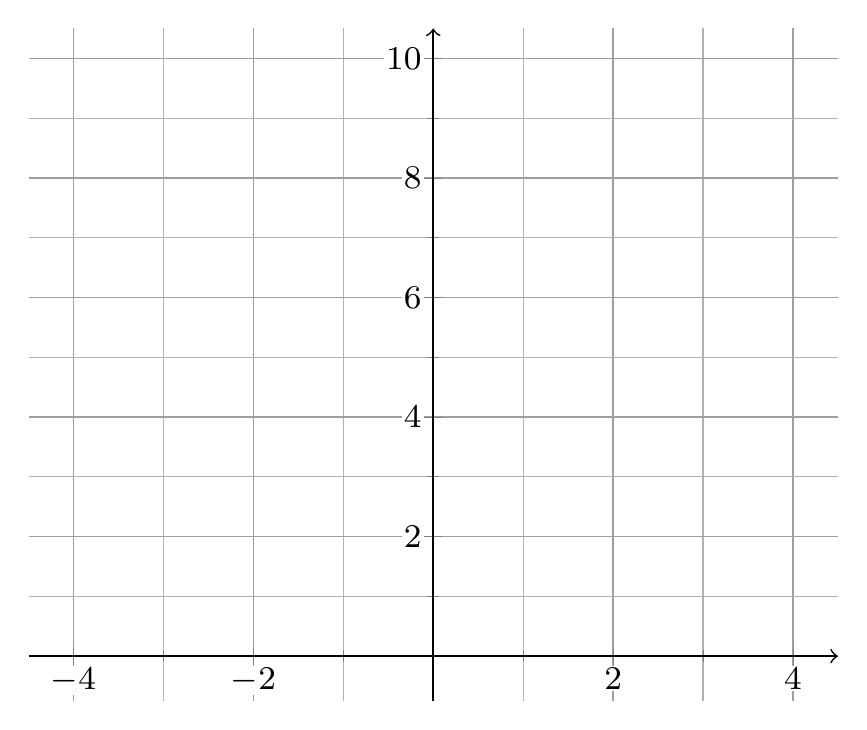
\begin{tikzpicture}[scale=1.5]
        \begin{axis}[
          grid=both, %major,minor
          grid style={line width=0.3pt, draw=gray!60},
          major grid style={line width=0.375pt, draw=gray!75},
          axis lines=center,
          axis line style={black,->},
          xmin=-4.5, xmax=4.5,
          ymin=-0.75, ymax=10.5,
          minor x tick num=1,
          minor y tick num=1,
          enlargelimits={value=0.5, auto},
          ticklabel style={font=\footnotesize,inner sep=0.5pt,fill=white,opacity=1.0, text opacity=1},
          ]
        \end{axis}
      \end{tikzpicture}
    \end{flushright}
  \end{minipage}
  \pagebreak
  
  \begin{ex*}
    Graph the exponential function
      \[y=\parens{\frac{1}{3}}^{x}\]
  \end{ex*}
  \begin{center}
    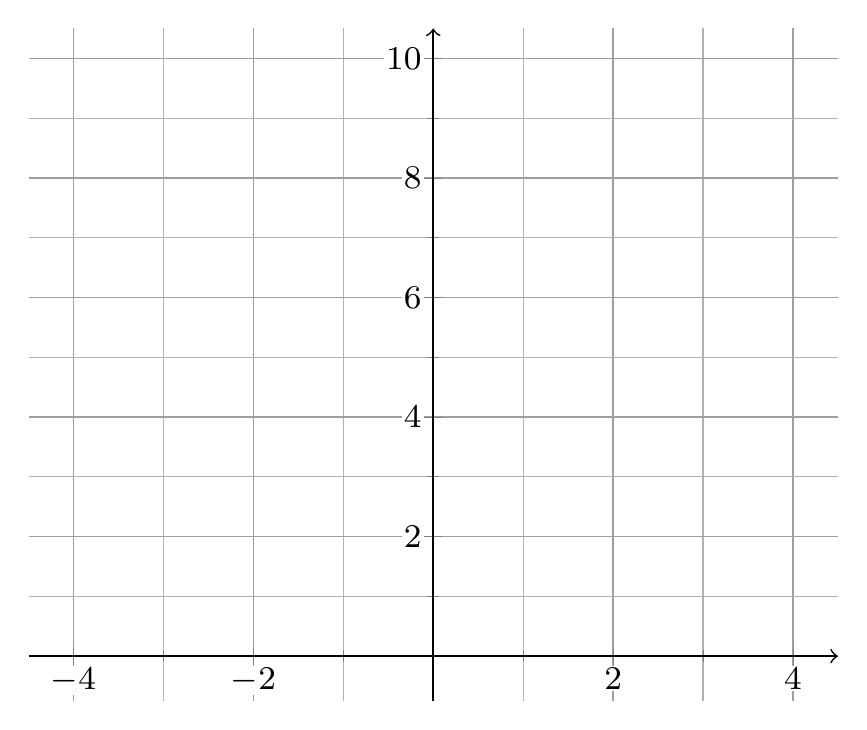
\begin{tikzpicture}[scale=1.5]
      \begin{axis}[
        grid=both, %major,minor
        grid style={line width=0.3pt, draw=gray!60},
        major grid style={line width=0.375pt, draw=gray!75},
        axis lines=center,
        axis line style={black,->},
        xmin=-4.5, xmax=4.5,
        ymin=-0.75, ymax=10.5,
        minor x tick num=1,
        minor y tick num=1,
        enlargelimits={value=0.5, auto},
        ticklabel style={font=\footnotesize,inner sep=0.5pt,fill=white,opacity=1.0, text opacity=1},
        ]
      \end{axis}
    \end{tikzpicture}
  \end{center}
  \vspace*{2\baselineskip}
  \begin{center}
    \fbox{\parbox{0.6\linewidth}{For an exponential function $a^x$, the function is
      \begin{itemize}
        \item increasing if $a>1$, and
        \item decreasing if $0<a<1$.
      \end{itemize}
    }}
  \end{center}
  \pagebreak

  \begin{ex*}
    Graph the exponential function
      \[y=\frac{1}{2}\parens{2}^x\]
  \end{ex*}
  \begin{center}
    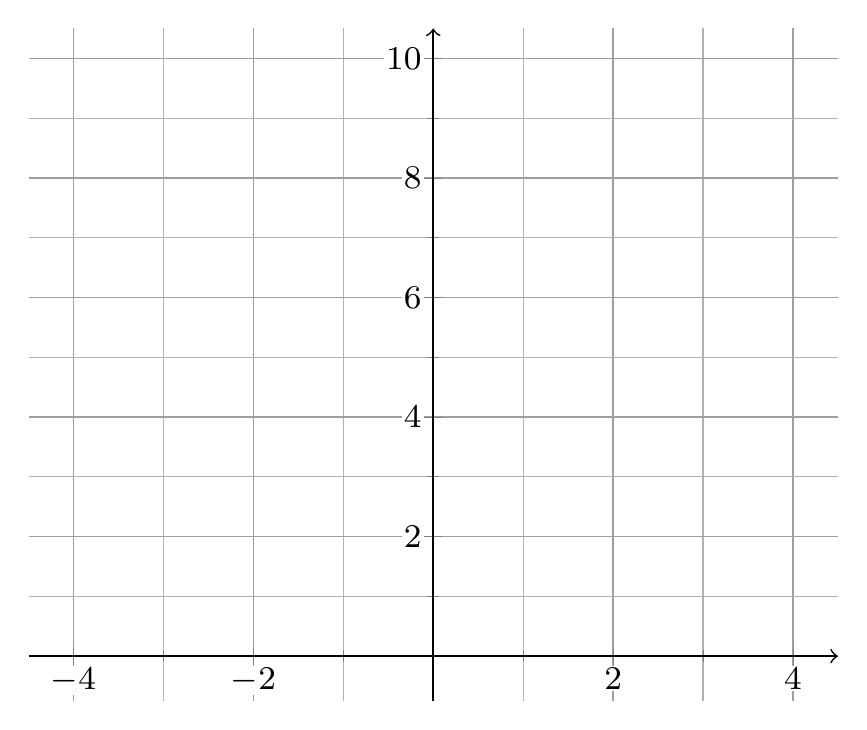
\begin{tikzpicture}[scale=1.5]
      \begin{axis}[
        grid=both, %major,minor
        grid style={line width=0.3pt, draw=gray!60},
        major grid style={line width=0.375pt, draw=gray!75},
        axis lines=center,
        axis line style={black,->},
        xmin=-4.5, xmax=4.5,
        ymin=-0.75, ymax=10.5,
        minor x tick num=1,
        minor y tick num=1,
        enlargelimits={value=0.5, auto},
        ticklabel style={font=\footnotesize,inner sep=0.5pt,fill=white,opacity=1.0, text opacity=1},
        ]
      \end{axis}
    \end{tikzpicture}
  \end{center}
  \pagebreak

  \begin{ex*}
    \textbf{Compound Interest:}\\
    If an initial principal $P$ is invested at a rate $r$ and compounded $n$ times a year, the future value in $t$ years is given by:
      \[A=P\parens{1+\frac{r}{n}}^{nt}\]
    Suppose that $\$800$ dollars is invested, and is compounded quarterly at a rate of $6\%$:
      \[A=800\parens{1.015}^{4t}\]
    Find the future value after 10 years.
  \end{ex*}
  \vspace*{\stretch{1}}
    
  \begin{ex*}
    \textbf{Compounded continuously:}\\
    A special function that frequently occurs in the context of exponential functions is 
      \[y=e^x\]
    where $e= 2.71828...$ (think irrational number like $\pi$). When an investment is compounded continuously, it's future value is given by
      \[A=Pe^{rt}\]
    Suppose that we invest $\$800$, compounded continuously at $6\%$. Find the future value in 10 years.
  \end{ex*}
  \vspace*{\stretch{1}}
  \pagebreak
  

  \pagebreak
\end{document}
